\documentclass[a4paper,12pt]{article}
\usepackage[left=2.5cm,right=2.5cm,top=2.5cm,bottom=2.5cm]{geometry} % Adjust page margins
\usepackage{xcolor,graphicx,framed}
\usepackage[normalem]{ulem}
\usepackage{amsmath}
\usepackage{cases}
\usepackage{gensymb}
\usepackage{chemmacros}
\setlength{\extrarowheight}{0.4cm}

\begin{document}

\newcommand{\HRule}{\rule{\linewidth}{0.4mm}} % Defines a new command for the horizontal lines, change thickness here

%----------------------------------------------------------------------------------------
%	HEADING SECTIONS
%----------------------------------------------------------------------------------------

\begin{minipage}{0.7\textwidth}
\begin{flushleft} 
\textsc{Universidad del Valle de Guatemala \\
Campus Central \\
Facultad de Ciencias y Humanidades \\
Departamento de Qu\'imica \\
Segundo ciclo, 2014 \\
Fisicoqu\'imica 1 \\
}
\end{flushleft}
\end{minipage}
~
\begin{minipage}{0.2\textwidth}
\begin{flushright}

\includegraphics[scale=0.3]{Logo_UVG} % Include a department/university logo
\end{flushright}
\end{minipage}\\

%----------------------------------------------------------------------------------------
%	TITLE SECTION
%----------------------------------------------------------------------------------------

\begin{center}
\HRule \\[0.4cm]
{ \bfseries Soluciones propuestas a los ejercicios en clase, 10}\\ % Title of your document
\HRule \\[0.4cm]
\end{center}

%----------------------------------------------------------------------------------------

\begin{enumerate}

 \item \textbf{\textit{(Chang 6.21)} Considere el siguiente sistema en equilibrio:}
$$\mbox{CaCO}_3\mbox{(s)}\;\ch{ <=> }\;\mbox{CaO(s)}+\mbox{CO}_2\mbox{(g)}$$
\textbf{?`Cu\'antas fases existen?} % Problema 6.21 de Chang

Si los dos compuestos s\'olidos forman una fase s\'olida homog\'enea, entonces el sistema tendr\'a 2 fases (la s\'olida y la gaseosa). Si no formaran una fase homog\'enea, entonces habr\'ian 3 fases.

 \item \textbf{\textit{(Chang 6.19)} Utilizar el diagrama de fases del agua para predecir la direcci\'on de los siguientes cambios:}
 \begin{enumerate}
  \item \textbf{en el punto triple del agua, la temperatura se reduce a presi\'on constante,}

El diagrama de fases del agua es el siguiente:

\begin{center}
 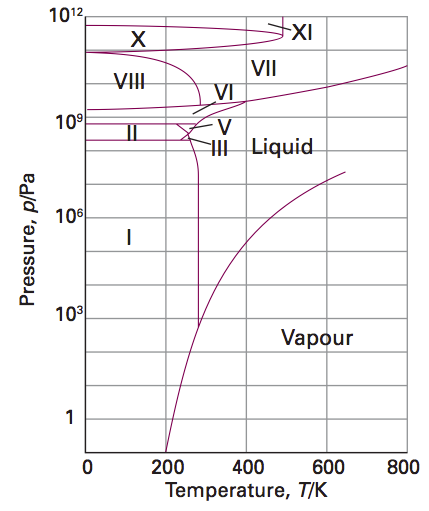
\includegraphics[scale=0.5]{figure9.png}
\end{center}

Si nos ubicamos en el punto triple del agua, al reducir la temperatura a presi\'on constante nos mover\'iamos en direcci\'on horizontal hacia la izquierda, por lo que el estado s\'olido se vuelve m\'as estable, mientras que el vapor y l\'iquido se volver\'ian inestables.

  \item \textbf{y en alg\'un punto a lo largo de la curva S-L del agua, aumenta la presi\'on a temperatura constante.}

Si nos ubicamos en la curva de S-L, o el l\'imite de fase entre los estados s\'olido y l\'iquido, al aumentar la presi\'on a temperatura constante nos mover\'iamos verticalmente hacia arriba, con lo que el estado l\'iquido se vuelve m\'as estable y el s\'olido inestable. Si aumentamos la presi\'on por varios \'ordenes de magnitud, entonces otros tipos de s\'olidos (o hielos) se vuelven la fase estable.

 \end{enumerate} % Problema 6.19 de Chang

 \item \textbf{\textit{(Chang 6.22)} En la siguiente figura se presenta un esquema aproximado del diagrama de fases del carbono. ?`Cu\'antos puntos triples tiene y cu\'ales son las fases que pueden coexistir en cada uno de ellos? ?`Cu\'al tiene mayor densidad: el grafito o el diamante? Se puede fabricar diamante sint\'etico a partir de grafito. Utilizando el diagrama de fases, ?`c\'omo har\'ia para fabricar diamante? (Ignorar la flecha en el diagrama.)}
\begin{center}
 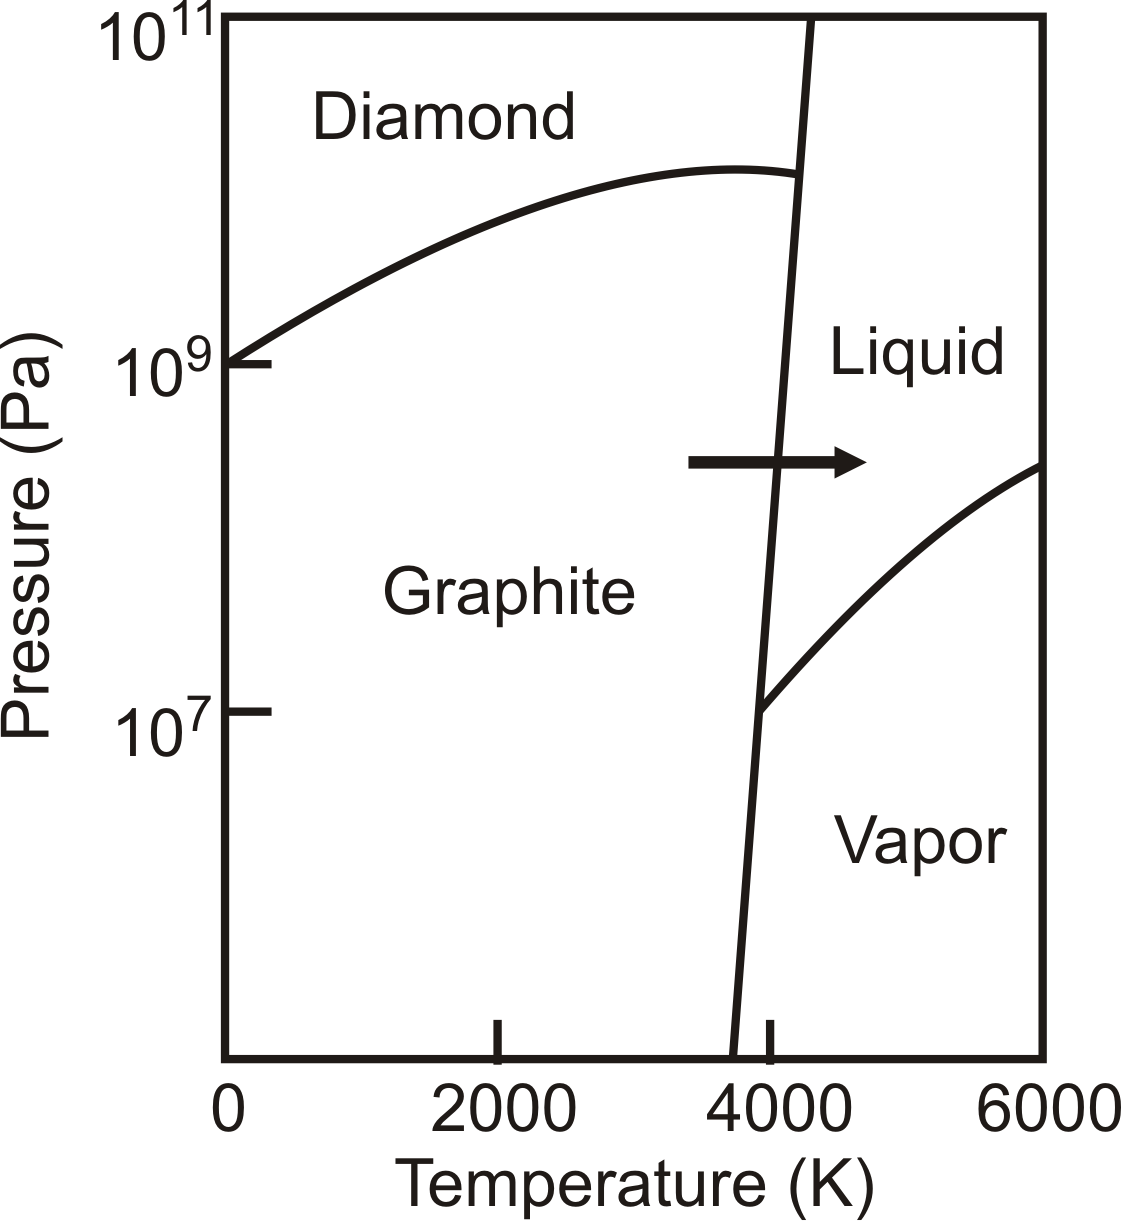
\includegraphics[scale=0.6]{figure4}
\end{center} % Problema 6.22 de Chang

N\'otese en la figura que se observan 2 puntos triples. En uno pueden coexistir el grafito, el l\'iquido y el vapor, mientras que en el otro pueden coexistir el diamante, el grafito y el l\'iquido. Considerando la relaci\'on inversa entre presi\'on y volumen de una sustancia (al aumental la presi\'on, el vol\'umen tiende a disminuir), se observa que el diamante es m\'as estable a presiones m\'as altas que el grafito, por lo que tendr\'ia menor volumen, as\'i que su densidad es mayor. Esta misma idea se podr\'ia usar para fabricar diamante a partir del grafito: aumentando la presi\'on a temperatura constante.

 \item \textbf{\textit{(McQuarrie 23-1)} Esbozar el diagrama de fase del ox\'igeno usando la siguiente informaci\'on: punto triple, $54.3\;\mbox{K}$ y $1.14\;\mbox{torr}$; punto cr\'itico, $154.6\;\mbox{K}$ y $37\,828\;\mbox{torr}$; punto de fusi\'on normal, $-218.4\celsius$; y punto de ebullici\'on normal, $-182.9\celsius$. ?`Se funde el ox\'igeno con presi\'on aplicada, de la misma forma que el agua?} % Problema 9-1

Usando los datos proporcionados, el esquema del diagrama de fase ser\'ia el siguiente (utilizando una escala logar\'itmica en el eje de la presi\'on, para permitir que aparezcan los puntos relevantes):

\begin{center}
 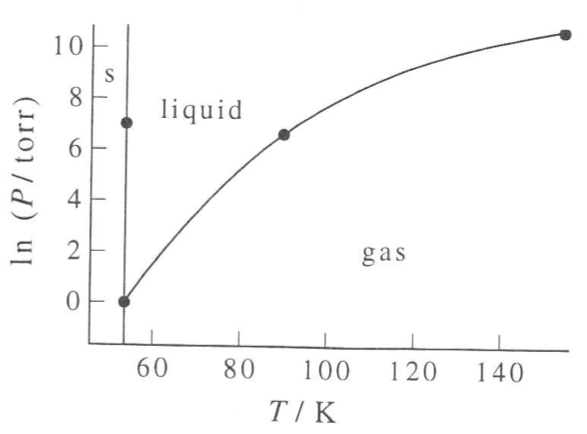
\includegraphics[scale=0.55]{figure6.png}
\end{center}

N\'otese que como el punto triple tiene una temperatura menor ($54.3\;\mbox{K}$) que la temperatura del punto de fusi\'on normal ($54.75\;\mbox{K}$), la pendiente de la curva del l\'imite de fase entre el s\'olido y el l\'iquido es positiva, as\'i que el ox\'igeno no se fundir\'ia con presi\'on aplicada, como sucede con el agua.

 \item \textbf{\textit{(McQuarrie 23-2)} Esbozar el diagrama de fase del $\mbox{I}_2$ usando la siguiente informaci\'on: punto triple, $113\celsius$ y $0.12\;\mbox{atm}$; punto cr\'itico, $512\celsius$ y $116\;\mbox{atm}$; punto de fusi\'on normal, $114\celsius$; punto de ebullici\'on normal, $184\celsius$; y la densidad del l\'iquido es mayor que la densidad del s\'olido.} % Problema 9-2

Usando los datos proporcionados, el esquema del diagrama de fase ser\'ia el siguiente (utilizando una escala logar\'itmica en el eje de la presi\'on, para permitir que aparezcan los puntos relevantes):

\begin{center}
 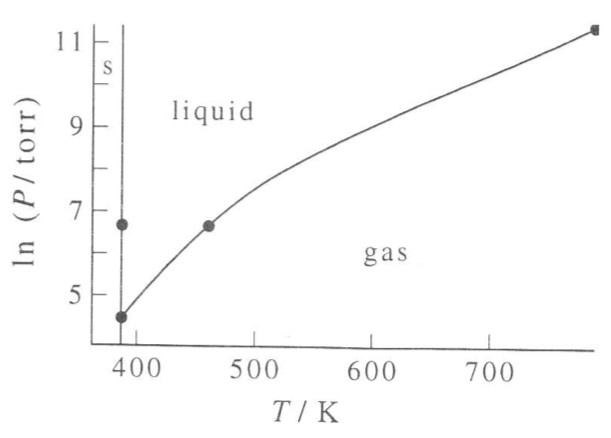
\includegraphics[scale=0.55]{figure7.png}
\end{center}

 \item \textbf{\textit{(McQuarrie 23-3)}  La siguiente figura muestra el diagrama de fase densidad-temperatura del benceno:}
\begin{center}
 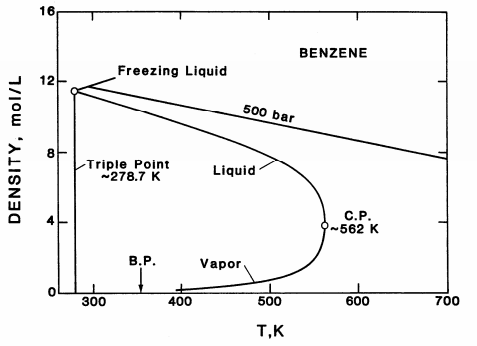
\includegraphics[scale=0.6]{figure5}
\end{center}
\textbf{Usando la siguiente informaci\'on para el punto triple y el punto cr\'itico, interpretar el diagrama de fase. ?`Por qu\'e el punto triple est\'a indicado como una l\'inea en este tipo de diagrama de fase?}

\begin{center}
\begin{tabular}{c|c c c c}
 &  &  & $\rho/\mbox{mol}\cdot\mbox{L}^{-1}$ & $\rho/\mbox{mol}\cdot\mbox{L}^{-1}$ \\
 & $T/\mbox{K}$ & $P/\mbox{bar}$ & Vapor & L\'iquido \\\hline
Punto triple & 278.680 & 0.04785 & 0.002074 & 11.4766 \\
Punto cr\'itico & 561.75 & 48.7575 & 3.90 & 3.90 \\
Punto de fusi\'on normal & 278.68 & 1.01325 &  &  \\
Punto de ebullici\'on normal & 353.240 & 1.01325 & 0.035687 & 10.4075  
\end{tabular}
\end{center} % Problema 9-3

En el punto cr\'itico, el gas y el l\'iquido se vuelven indistinguibles, por lo que esperar\'iamos que conforme nos acercamos a la temperatura del punto cr\'itico, las densidades del l\'iquido y del gas se acercan entre s\'i. En el punto triple, las densidades del l\'iquido y el vapor difieren por varios ordenes de magnitud, pero no hay restricci\'on de cantidades en cada fase, por lo que dependiendo las proporciones, la densidad del sistema puede tener cualquier valor entre la densidad del gas y la densidad del l\'iquido, por eso se observa una l\'inea para el punto triple en este diagrama.

 \item \textbf{\textit{(McQuarrie 23-7 y 23-8)} La presi\'on de vapor del metanol a lo largo de toda la curva de co-existencia l\'iquido-vapor puede ser expresada de manera precisa por la f\'ormula emp\'irica:}

\begin{center}
\begin{tabular}{r c l}
$\ln(P/\mbox{bar})$ & $=$ & $-10.752849/x+16.758207-3.603425x$\\
& & $\quad +4.373232x^2-2.381377x^3+4.572199(1-x)^{1.70}$
\end{tabular}
\end{center} 
\textbf{donde $x=T/T_c$ y $T_c=512.60\;\mbox{K}$. Usar esta f\'ormula para mostrar que el punto de ebullici\'on normal del metanol es $337.67\;\mbox{K}$ y el punto de ebullici\'on est\'andar $337.33\;\mbox{K}$.} % Problema 9-7 y 9-8

La curva de presi\'on de vapor relaciona el l\'imite de fase entre el l\'iquido y el vapor. El punto de ebullici\'on normal es el punto sobre esta curva en el cual la presi\'on vale $1\;\mbox{atm}$ (mientras que el punto de ebullici\'on est\'andar es el punto sobre la curva en el cual la presi\'on vale $1\;\mbox{bar}$), as\'i que para mostrar que la temperatura del punto de ebullici\'on normal es $337.67\;\mbox{K}$ se puede sustituir los valores en la ecuaci\'on y mostrar que la satisfacen. 

Para el punto de ebullici\'on normal, el lado izquierdo ser\'ia:
$$\ln (P/\mbox{bar})=\ln\left(1\;\mbox{atm}\left(\frac{1.01325\;\mbox{bar}}{1\;\mbox{atm}}\right)/\mbox{bar}\right)=0.0132$$
Para el lado derecho, tenemos que $x=T/T_c=(337.67\;\mbox{K})/(512.60\;\mbox{K})$, as\'i que:

\begin{tabular}{r c l}
$-10.752849/\left(\frac{337.67}{512.60}\right)+16.758207-3.603425(\frac{337.67}{512.60})$ & & \\
$+4.373232(\frac{337.33}{512.60})^2-2.381377(\frac{337.67}{512.60})^3+4.572199\left(1-\frac{337.67}{512.60}\right)^{1.70}$ & $=$ & $0.0132$ 
\end{tabular}

Para el punto de ebullici\'on est\'andar, el lado izquierdo ser\'ia:
$$\ln (P/\mbox{bar})=\ln (1\;\mbox{bar}/\mbox{bar})=0$$
Para el lado derecho, tenemos que $x=T/T_c=(337.33\;\mbox{K})/(512.60\;\mbox{K})$, as\'i que:

\begin{tabular}{r c l}
$-10.752849/\left(\frac{337.33}{512.60}\right)+16.758207-3.603425(\frac{337.33}{512.60})$ & & \\
$+4.373232(\frac{337.33}{512.60})^2-2.381377(\frac{337.33}{512.60})^3+4.572199\left(1-\frac{337.33}{512.60}\right)^{1.70}$ & $=$ & $0$
\end{tabular}

\end{enumerate}
 
\end{document}
